\section{Harder, better, faster, stronger: enrolling other nodes with MPI}

\begin{frame}{MPI?}
	\begin{itemize}
		\item MPI = "message passing interface." It is a communication protocol for programming parallel computers. It defines a common and portable API.
		\item It provides different kinds of communication (point-to-point, collective, one-sided, ...), management, and parallel I/O.
		\item Consequence: sharing the workload is now \textbf{explicit} (and communication is a bottleneck)!
		\item The API is similar to the sockets (\textit{i.e.}, \cdx{open} / \cdx{send} / \cdx{recv} / \cdx{close}), with some improvements:\begin{center}
			\begin{tikzpicture}
				\draw[latex-latex] (-.25,-.75) -- node[midway,left]{\small \cdx{mpirun -np 3}} + (0,1.5);
				\draw[|-|] (0,.75)  node[right=.2cm,draw,fill=white]{\small \cdx{MPI\_Init}}-- +(6.6,0) node[left=.2cm,draw,fill=white]{\small \cdx{MPI\_Finalize}}; 
				\draw[|-|]  (0,0) node[right=.2cm,draw,fill=white]{\small \cdx{MPI\_Init}}-- +(6.6,0) node[left=.2cm,draw,fill=white]{\small \cdx{MPI\_Finalize}};  
				\draw[|-|]  (0,-.75) node[right=.2cm,draw,fill=white]{\small \cdx{MPI\_Init}}-- +(6.6,0) node[left=.2cm,draw,fill=white]{\small \cdx{MPI\_Finalize}}; 
				\begin{scope}[decoration={
						markings,
						mark=at position 0.65 with {\arrow{latex}}}
					] 
					\draw[postaction={decorate},blue] (2.25,.75) node[draw,fill=white]{\small s} -- +(0,-.75) node[draw,fill=white]{\small r};
					\draw[red] (2.75,0) node[draw,fill=white]{c};
					\draw[postaction={decorate},blue] (2.75,.75) node[draw,fill=white]{\small s} -- +(0,-1.5) node[draw,fill=white]{\small r};
					\draw[postaction={decorate},blue] (3.25,0) node[draw,fill=white]{\small s} -- +(0,.75) node[draw,fill=white]{\small r};
					\draw[red] (3.25,-.75) node[draw,fill=white]{c};
					\draw[postaction={decorate},blue] (3.75,-.75) node[draw,fill=white]{\small s} -- +(0,1.5) node[draw,fill=white]{\small r};
				\end{scope}
			\end{tikzpicture}
		\end{center}
		\item For maximal performances, MPI can be combined with OpenMP.
	\end{itemize}
\end{frame}

\begin{frame}[fragile]{Hello, world!}
\begin{ccode}
#include <mpi.h>
#include <stdio.h>

int main(int argc, char* argv[]) {
	MPI_Init(&argc, &argv);
	int rank, size, len;
	char name[MPI_MAX_PROCESSOR_NAME];
	MPI_Comm_rank(MPI_COMM_WORLD, &rank);
	MPI_Comm_size(MPI_COMM_WORLD, &size);
	MPI_Get_processor_name(name, &len);
	printf("Rank=%d, size=%d (node=%s)\n", rank, size, name);
	MPI_Finalize();
	return 0;
}
\end{ccode}

Processes are grouped into \textbf{communicators}, \textit{i.e.}, a group of processes that can communicate. In such group, each process is assigned a (unique) \textbf{rank}. Default is \cdx{MPI\_COMM\_WORLD} (all processes). The size of the communicator gives the number of processes in this communicator.
\end{frame}

\begin{frame}[fragile]{Compile and run}
	\begin{itemize}
		\item MPI is generally not installed by default and comes in different flavors (implementations). You can install \cdx{openmpi} on your computer.
		\item There is a specific wrapper for the compilation \cdx{mpi[xx]} (which just add the relevant options), \textit{e.g.},\begin{textcode}
mpicc -o hello hello.c
		\end{textcode}
	\item To use the application, you must use the launcher, \cdx{mpirun}, with the number of processes as argument:\begin{textcode}
mpirun -np 2 ./hello
	\end{textcode}
\item With the example given in previous slide, the output is\begin{textcode}
Rank=0, size=2 (node=raspi-cluster-master)
Rank=1, size=2 (node=raspi-cluster-master)
\end{textcode}
	\end{itemize}
\end{frame}

\begin{frame}{Sending}
	MPI passes data in the form of \textbf{messages}. They may be divided in two parts:\begin{enumerate}
		\item Message content: the data to be sent (MPI suppose it is array-like),
		\item The ``envelope'': to which process the message is addressed.
	\end{enumerate}
\begin{center}
	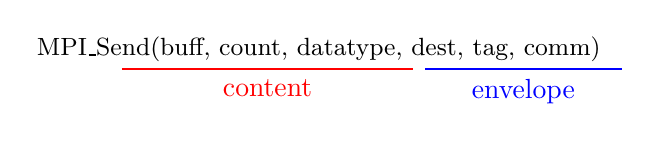
\begin{tikzpicture}
		\draw (0,0) node{\small \cdx{MPI\_Send(buff, count, datatype, dest, tag, comm)}};
		\draw[thick,red] (-2.5,-.25) -- +(3.7,0) node[midway,below]{content};
		\draw[thick,blue] (1.35,-.25) -- +(2.5,0) node[midway,below]{envelope};
	\end{tikzpicture}
\end{center}
The message \cdx{tag} helps to discriminate between different messages addressed to the same process. It is user defined.
\end{frame}

\begin{frame}[fragile]{Sending}
	Sending data to a specific process may be done through one variant of
	\begin{ccode}
MPI_Send(
	void* buff,      // data
	int count,       // number of element to be sent
	MPI_Datatype dt, // type of an element
	int dest,        // recipient (rank)
	int tag,         // type of message
	MPI_Comm c,      // communicator
);
	\end{ccode}
There is also \cdx{MPI\_Isend}, which is \textbf{immediate} (non-blocking). \cdx{dt} may be\begin{itemize}
	\item \cdx{MPI\_CHAR} / \cdx{MPI\_UNSIGNED\_CHAR} (or \cdx{MPI\_BYTE}),
	\item \cdx{MPI\_INT} / \cdx{MPI\_UNSIGNED\_INT},
	\item \cdx{MPI\_LONG} / \cdx{MPI\_UNSIGNED\_LONG},
	\item \cdx{MPI\_FLOAT} / \cdx{MPI\_DOUBLE},
	\item \cdx{MPI\_PACKED} (\textit{i.e.}, \cdx{struct}).
\end{itemize}
\end{frame}

\begin{frame}[fragile]{Receiving}
	Receiving data to a specific process may be done through one variant of
	\begin{ccode}
MPI_Recv(
	void* buff,      // data
	int count,       // number of element to be sent
	MPI_Datatype dt, // type of an element
	int source,      // sender (rank)
	int tag,         // type of message
	MPI_Comm c,      // communicator
	MPI_Status* s    // information on the message
);
	\end{ccode}
	Note that for a communication to succeed, the following should be met:\begin{enumerate}
		\item The same communicator must be used
		\item Source and destination rank must match
		\item The tag must match
		\item The buffer should be large enough on the receive side.
	\end{enumerate}
	Note that \cdx{count} is the \textbf{maximal} number of elements that can be received.
	
\end{frame}

\begin{frame}{Example (ring communication)}
	Ring communication (sent to its next neighbor in the ring, receive from its previous). The goal is, \textit{e.g.}, that every process should have the sum of the ranks at the end:\begin{enumerate}
		\item Set \cdx{sum = 0}, and \cdx{send\_buffer = rank},
		\item Send the buffer to next neighbor, 
		\item Get from the previous in \cdx{receive\_buffer}, adds it to \cdx{sum},
		\item \cdx{send\_buffer = receive\_buffer},
		\item Repeat from step 2 until all ranks have been propagated along the ring.
	\end{enumerate}
\begin{center}
	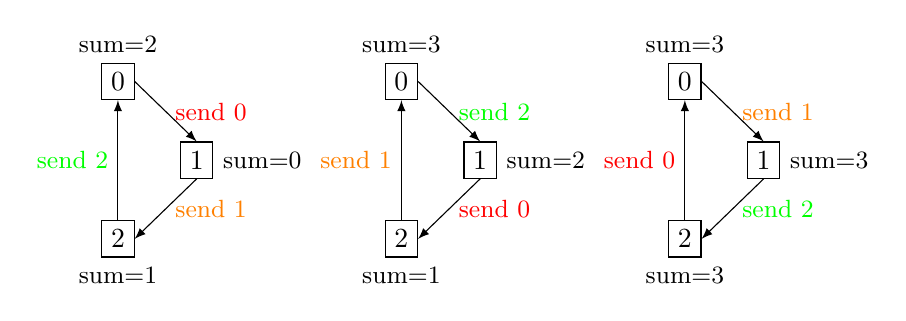
\begin{tikzpicture}[scale=.6]
		\begin{scope}
			\node (x) {};
			\node[above of=x, draw] (x0)  {0};
			\draw (x0.north) node[above] {\small \cdx{sum=2}};
			\node[right of=x,draw] (x1) {1};
			\draw (x1.east) node[right] {\small \cdx{sum=0}};
			\node[below of=x,draw] (x2) {2};
			\draw (x2.south) node[below] {\small \cdx{sum=1}};
			\draw[-latex] (x0.east) -- node[midway,right,red]{\small send 0} (x1.north);
			\draw[-latex] (x1.south) -- (x2.east) node[midway,right,orange]{\small send 1};
			\draw[-latex] (x2.north) -- (x0.south) node[midway,left,green]{\small send 2};
		\end{scope}
	\begin{scope}[xshift=6cm]
	\node (x) {};
	\node[above of=x, draw] (x0)  {0};
	\draw (x0.north) node[above] {\small \cdx{sum=3}};
	\node[right of=x,draw] (x1) {1};
	\draw (x1.east) node[right] {\small \cdx{sum=2}};
	\node[below of=x,draw] (x2) {2};
	\draw (x2.south) node[below] {\small \cdx{sum=1}};
	\draw[-latex] (x0.east) -- node[midway,right,green]{\small send 2} (x1.north);
	\draw[-latex] (x1.south) -- (x2.east) node[midway,right,red]{\small send 0};
	\draw[-latex] (x2.north) -- (x0.south) node[midway,left,orange]{\small send 1};
\end{scope}
\begin{scope}[xshift=12cm]
	\node (x) {};
	\node[above of=x, draw] (x0)  {0};
	\draw (x0.north) node[above] {\small \cdx{sum=3}};
	\node[right of=x,draw] (x1) {1};
	\draw (x1.east) node[right] {\small \cdx{sum=3}};
	\node[below of=x,draw] (x2) {2};
	\draw (x2.south) node[below] {\small \cdx{sum=3}};
	\draw[-latex] (x0.east) -- node[midway,right,orange]{\small send 1} (x1.north);
	\draw[-latex] (x1.south) -- (x2.east) node[midway,right,green]{\small send 2};
	\draw[-latex] (x2.north) -- (x0.south) node[midway,left,red]{\small send 0};
\end{scope}
	\end{tikzpicture}
\end{center}
\end{frame}

\begin{frame}[fragile]{Example (synchronous)}
\begin{ccode}
send_buffer = rank;
for(int i=0; i < comm_size; i++) {
	if (rank % 2 == 0) { // WHY?
		MPI_Send(&send_buffer, 1, MPI_INT, next_rank, rank, 
			MPI_COMM_WORLD);
		MPI_Recv(&receive_buffer, 1, MPI_INT, prev_rank, prev_rank, 
			MPI_COMM_WORLD, MPI_STATUS_IGNORE);
	} else {
		MPI_Recv(&receive_buffer, 1, MPI_INT, prev_rank, prev_rank, 
			MPI_COMM_WORLD, MPI_STATUS_IGNORE);
		MPI_Send(&send_buffer, 1, MPI_INT, next_rank, rank, 
			MPI_COMM_WORLD);
	}
	sum += receive_buffer;
	send_buffer = receive_buffer;
}
\end{ccode}
\end{frame}

\begin{frame}[fragile]{Example (asynchronous)}
Both asynchronous call:
\begin{ccode}
MPI_Request requests[2];
MPI_Isend(&send_buffer, 1, MPI_INT, next_rank, rank, 
	MPI_COMM_WORLD, &requests[0]);
MPI_Irecv(&receive_buffer, 1, MPI_INT, prev_rank, prev_rank, 
	MPI_COMM_WORLD, &requests[1]);
MPI_Waitall(2, requests, MPI_STATUS_IGNORE); // barrier
\end{ccode}
or asynchronous sent followed by synchronous receive:
\begin{ccode}
MPI_Request request;
MPI_Isend(&send_buffer, 1, MPI_INT, next_rank, rank, 
	MPI_COMM_WORLD, &request);
MPI_Recv(&receive_buffer, 1, MPI_INT, prev_rank, prev_rank, 
	MPI_COMM_WORLD, MPI_STATUS_IGNORE);
MPI_Wait(&request, MPI_STATUS_IGNORE); // not required
\end{ccode}

\end{frame}

\begin{frame}[fragile]{Example: ping-pong}
\begin{ccode}
long N = 2 << i;
double* A = calloc(N, sizeof(double));
elapsed = MPI_Wtime();
for(int k=0; k < N_PING_PONG; k++) {
	if (rank == 0) {
		MPI_Send(A, N, MPI_DOUBLE, 1, 0, 
			MPI_COMM_WORLD);
		MPI_Recv(A, N, MPI_DOUBLE, 1, 0, 
			MPI_COMM_WORLD, MPI_STATUS_IGNORE);
	} else {
		MPI_Recv(A, N, MPI_DOUBLE, 0, 0, 
			MPI_COMM_WORLD, MPI_STATUS_IGNORE);
		MPI_Send(A, N, MPI_DOUBLE, 0, 0, 
			MPI_COMM_WORLD);
	}
}
elapsed = MPI_Wtime() - elapsed;
\end{ccode}
Elapsed time depends on the amount of data and asymptotically tend to the bandwith.
\end{frame}

\begin{frame}{Example: ping-pong}
	\begin{figure}
		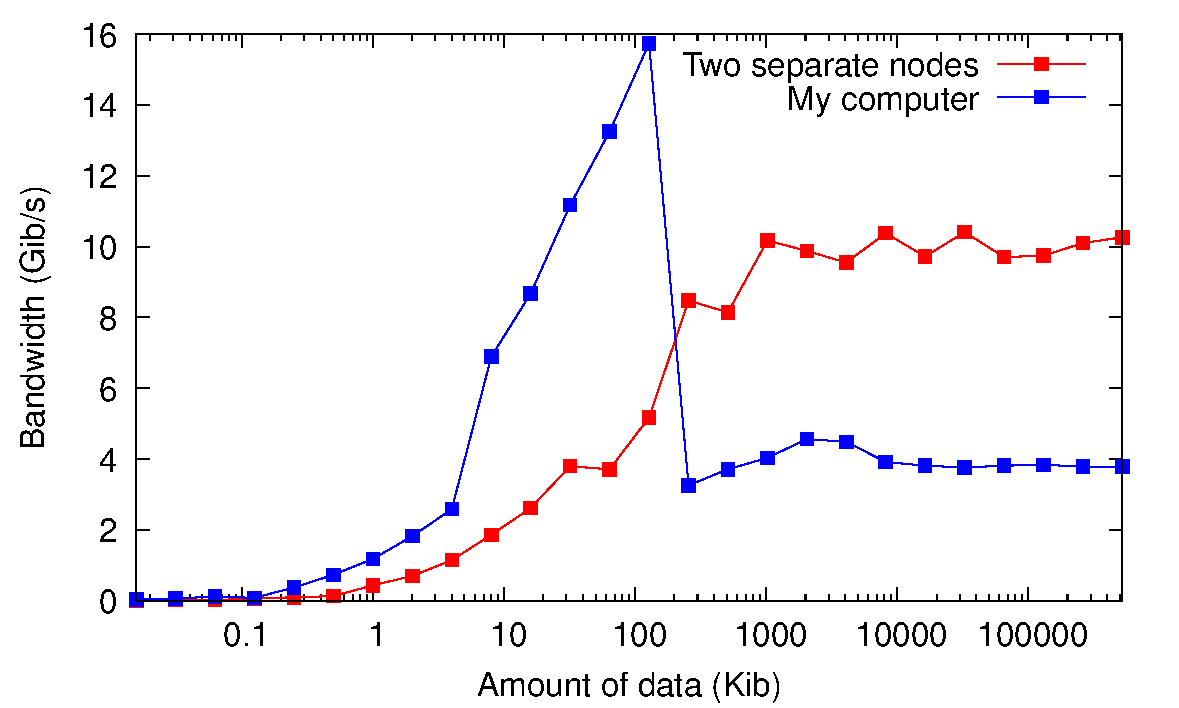
\includegraphics[width=.85\textwidth]{im/result_MPI_ping}
		\caption{Bandwidth, as measured by the ping-pong example, in two different configurations}
	\end{figure}
What (the hell!) did happen in both cases?
\end{frame}

\begin{frame}{Other ways to communicate}
	\begin{center}
		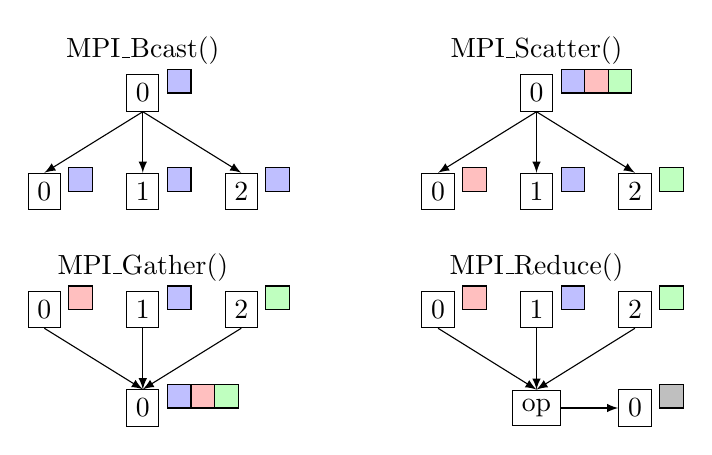
\begin{tikzpicture}[node distance=1.25cm]
			\begin{scope}
				\node[draw] (x0) {0};
				\draw (x0.north) node[above]{\cdx{MPI\_Bcast()}};
				\draw[fill=blue!25] (x0.east) ++(.1,0) rectangle ++(.3,.3);
				\node[below of=x0,draw] (y1) {1};
				\draw[fill=blue!25] (y1.east) ++(.1,0) rectangle ++(.3,.3);
				\node[left of=y1,draw] (y0) {0};
				\draw[fill=blue!25] (y0.east) ++(.1,0) rectangle ++(.3,.3);
				\node[right of=y1,draw] (y2) {2};
				\draw[fill=blue!25] (y2.east) ++(.1,0) rectangle ++(.3,.3);
				\draw[-latex] (x0.south) --(y0.north);
				\draw[-latex] (x0.south) --(y1.north);
				\draw[-latex] (x0.south) --(y2.north);
			\end{scope}
		\begin{scope}[xshift=5cm]
		\node[draw] (x0) {0};
		\draw (x0.north) node[above]{\cdx{MPI\_Scatter()}};
		\draw[fill=blue!25] (x0.east) ++(.1,0) rectangle ++(.3,.3);
		\draw[fill=red!25] (x0.east) ++(.4,0) rectangle ++(.3,.3);
		\draw[fill=green!25] (x0.east) ++(.7,0) rectangle ++(.3,.3);
		\node[below of=x0,draw] (y1) {1};
		\draw[fill=blue!25] (y1.east) ++(.1,0) rectangle ++(.3,.3);
		\node[left of=y1,draw] (y0) {0};
		\draw[fill=red!25] (y0.east) ++(.1,0) rectangle ++(.3,.3);
		\node[right of=y1,draw] (y2) {2};
		\draw[fill=green!25] (y2.east) ++(.1,0) rectangle ++(.3,.3);
		\draw[-latex] (x0.south) --(y0.north);
		\draw[-latex] (x0.south) --(y1.north);
		\draw[-latex] (x0.south) --(y2.north);
	\end{scope}
\begin{scope}[yshift=-4cm]
\node[draw] (x0) {0};
\draw[fill=blue!25] (x0.east) ++(.1,0) rectangle ++(.3,.3);
\draw[fill=red!25] (x0.east) ++(.4,0) rectangle ++(.3,.3);
\draw[fill=green!25] (x0.east) ++(.7,0) rectangle ++(.3,.3);
\node[above of=x0,draw] (y1) {1};
\draw (y1.north) node[above]{\cdx{MPI\_Gather()}};
\draw[fill=blue!25] (y1.east) ++(.1,0) rectangle ++(.3,.3);
\node[left of=y1,draw] (y0) {0};
\draw[fill=red!25] (y0.east) ++(.1,0) rectangle ++(.3,.3);
\node[right of=y1,draw] (y2) {2};
\draw[fill=green!25] (y2.east) ++(.1,0) rectangle ++(.3,.3);
\draw[-latex] (y0.south) --(x0.north);
\draw[-latex] (y1.south) --(x0.north);
\draw[-latex] (y2.south) --(x0.north);
\end{scope}
\begin{scope}[yshift=-4cm,xshift=5cm]
	\node[draw] (x0) {op};
	\node[right of=x0,draw] (x1) {0};
	\draw[fill=black!25] (x1.east) ++(.1,0) rectangle ++(.3,.3);
	\node[above of=x0,draw] (y1) {1};
	\draw (y1.north) node[above]{\cdx{MPI\_Reduce()}};
	\draw[fill=blue!25] (y1.east) ++(.1,0) rectangle ++(.3,.3);
	\node[left of=y1,draw] (y0) {0};
	\draw[fill=red!25] (y0.east) ++(.1,0) rectangle ++(.3,.3);
	\node[right of=y1,draw] (y2) {2};
	\draw[fill=green!25] (y2.east) ++(.1,0) rectangle ++(.3,.3);
	\draw[-latex] (y0.south) --(x0.north);
	\draw[-latex] (y1.south) --(x0.north);
	\draw[-latex] (y2.south) --(x0.north);
	\draw[-latex] (x0.east) --(x1.west);
\end{scope}
		\end{tikzpicture}
	\end{center}
... And others (asynchronous \cdx{I*}, All-to-all \cdx{All*}, vectors \cdx{*v}, ...).
\end{frame}

\begin{frame}{Results}
	\begin{figure}
		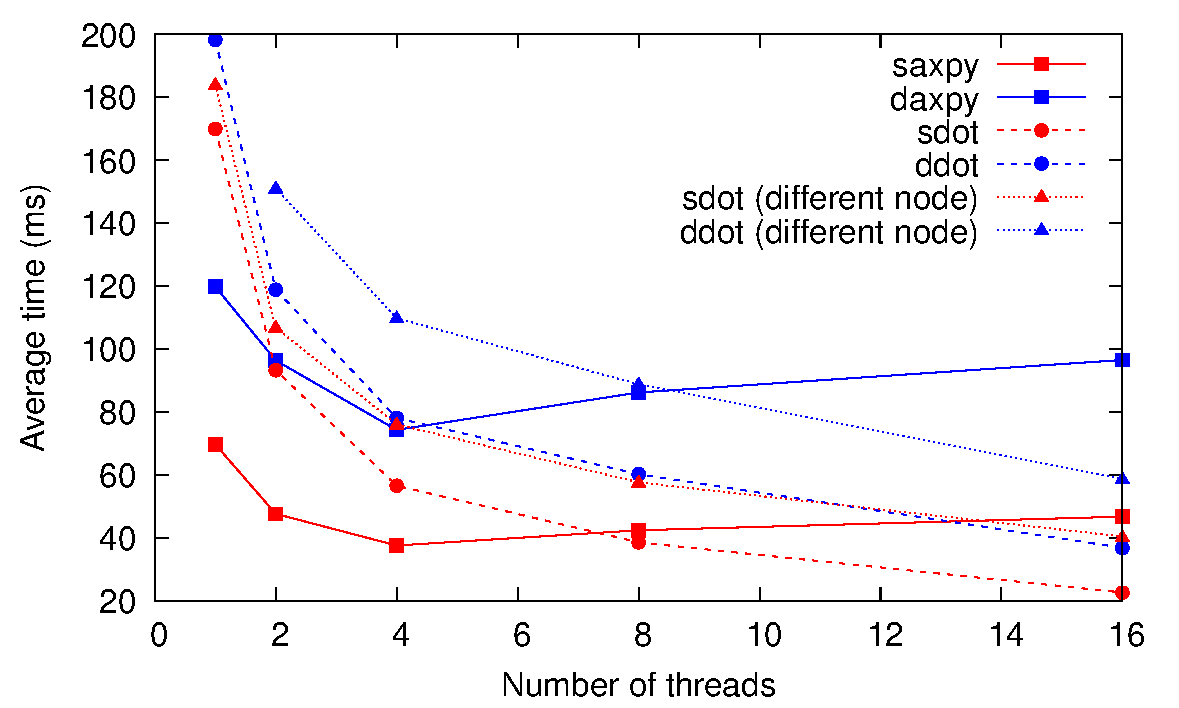
\includegraphics[width=.75\textwidth]{im/result_MPI}
		\caption{Results ($2^{24}$ numbers) with \cdx{-N 1000} and different number of processes.}
	\end{figure}
\begin{itemize}
	\item Not so good in general.
	\item Again, more interesting for \cdx{*dot} (more work intensive) than for \cdx{*axpy} (bandwidth limited).
	\item Thanks to Infiniband, not so much impact when different nodes are used.
\end{itemize}
\end{frame}